% Generated by thesis/ch7/exp2/networks.py -- do not edit by hand.
\begin{sidewaysfigure}
  \centering
  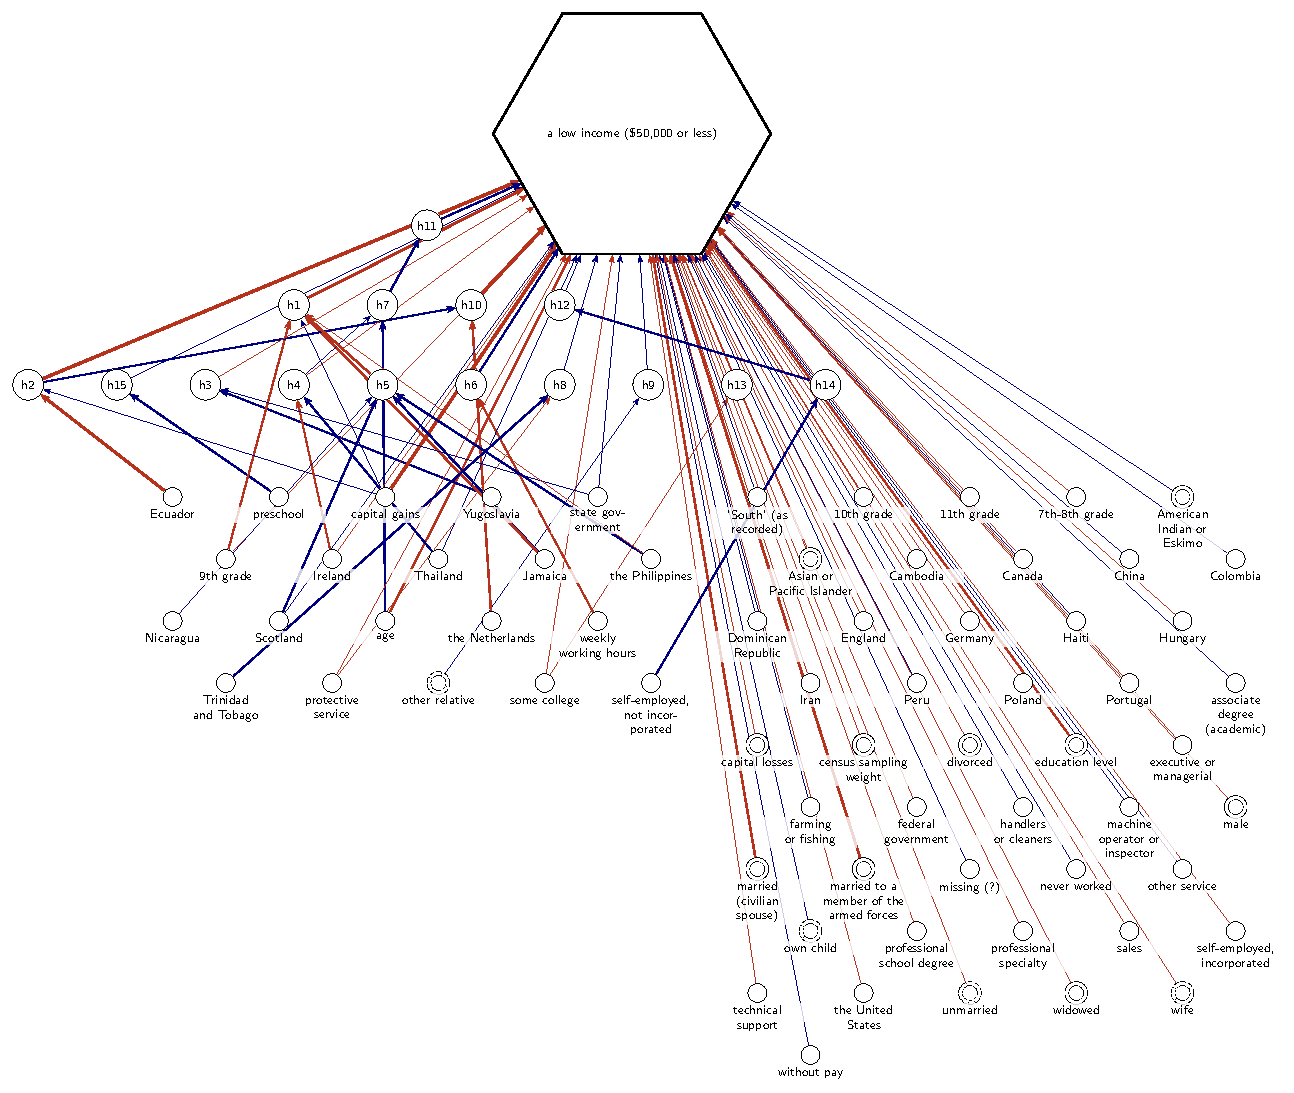
\includegraphics[width=\textheight,height=0.78\textwidth,keepaspectratio]{figures/exp2/networks/adult-s5-raw}
  \caption{Adult, seed 5 (adult-s5): the network as trained, before any explanation, in full. Inputs at the bottom (every input column its own node), hidden units by depth, the output at the top; 66 of 107 input columns are connected, with 15 hidden units and 95 enabled connections. Blue: positive weight (raises the score); red: negative weight (lowers it); thicker: larger weight. Orange outline and up arrow: raises the final prediction; teal and down arrow: lowers it; grey and double arrow: depends. Not used (no connection; 41 columns): missing (?), local government, private, doctorate, high-school graduate, master's degree, 12th grade (no diploma), 1st-4th grade, 5th-6th grade, associate degree (vocational), bachelor's degree, married, spouse absent, never married, separated, administrative or clerical, transport or moving, armed forces, craft or repair, private household service, husband, not in a family, Black, other race, White, missing (?), France, Greece, Guatemala, Honduras, Hong Kong, India, Italy, Japan, Laos, Mexico, outlying US territories (Guam, US Virgin Islands), Puerto Rico, Taiwan, Vietnam, Cuba and El Salvador.}
  \label{fig:exp2-net-adult-s5-raw}
\end{sidewaysfigure}
